% Outline
% 
% Section 1
%   History of GeoSPARWL 1.0
% Section 2
%   motivation to update the spec
% Section 3
%   GeoSPARQL 1.1 additions
%       motivation, and expected use, of new spatial functions. In particular, why in GeoSPARQL when aggregations etc. can be performed elsewhere?
%       Spatial Measure
% Section 4
%       new profile preentation
%       new URI regimes etc
% Section 5
%       expected changed use modes
\documentclass[runningheads]{llncs}

\usepackage{graphicx}
\usepackage[hidelinks]{hyperref,xcolor}
\renewcommand\UrlFont{\color{blue}\rmfamily}

\begin{document}

\title{GeoSPARQL 1.1: an almost decadal update to the most important geospatial LOD standard}
\titlerunning{GeoSPARQL 1.1}

\author{
    Nicholas J. Car\inst{1,2}\orcidID{0000-0002-8742-7730} \and \\
    Timo Homburg\inst{3}\orcidID{1111-2222-3333-4444} % \and \\
    % Third Author\inst{3}\orcidID{2222-3333-4444-5555}
}

\authorrunning{Car N.J. et al.}

\institute{SURROUND Australia Pty Ltd., Brisbane Australia \and
Australian National University, Canberra Australia \and Mainz University Of Applied Sciences, Germany
\email{nicholas.car@surroundaustralia.com, timo.homburg@hs-mainz.de}\\
\url{https://surroundaustralia.com} \and
ABC Institute, Rupert-Karls-University Heidelberg, Heidelberg, Germany\\
\email{\{abc,lncs\}@uni-heidelberg.de}}

\maketitle

\begin{abstract}
The Open Geospatial Consortium published the GeoSPARQL 1.0 standard in 2012 containing multiple 
parts that define ``SPARQL extension functions'', ``RIF rules'', ``an RDF/OWL ontology for 
information based on the General Feature Model'' and supporting vocabularies, all for Semantic 
Web spatial data.\\

In the 8+ years since its publication, GeoSPARQL has become the most important spatial Semantic 
Web standard, as judged by references to it in other Semantic Web standards and its wide use in 
Semantic Web data.\\

An update to the standard was proposed in 2019 to deliver GeoSPARQL 1.1 in 2021 with a charter to: 
handle outstanding change requests and source new ones from the GeoSPARQL user community as well 
to ``better present'' the standard, that is to better link all the standard’s parts and better 
document \& exemplify elements. Expected updates included possible alignments to other ontologies, 
possible handling of new spatial referencing systems, new geometry representations and new artifact 
presentation.\\

In this paper, we will discuss the submitted change requests and resulting updates to the standard. 
We will also discuss the theory behind updates and our expectations for GeoSPARQL 1.1's use.

\keywords{GeoSPARQL  \and GeoSPARQL 1.1 \and spatial \and geospatial \and Semantic Web \and RDF \and OWL \and OGC \and Open Geospatial Consortuim \and standard.}
\end{abstract}


\section{First Section}
\subsection{A Subsection Sample}
Please note that the first paragraph of a section or subsection is
not indented. The first paragraph that follows a table, figure,
equation etc. does not need an indent, either.

Subsequent paragraphs, however, are indented.

\subsubsection{Sample Heading (Third Level)} Only two levels of
headings should be numbered. Lower level headings remain unnumbered;
they are formatted as run-in headings.

\paragraph{Sample Heading (Fourth Level)}
The contribution should contain no more than four levels of
headings. Table~\ref{tab1} gives a summary of all heading levels.

\begin{table}
\caption{Table captions should be placed above the
tables.}\label{tab1}
\begin{tabular}{|l|l|l|}
\hline
Heading level &  Example & Font size and style\\
\hline
Title (centered) &  {\Large\bfseries Lecture Notes} & 14 point, bold\\
1st-level heading &  {\large\bfseries 1 Introduction} & 12 point, bold\\
2nd-level heading & {\bfseries 2.1 Printing Area} & 10 point, bold\\
3rd-level heading & {\bfseries Run-in Heading in Bold.} Text follows & 10 point, bold\\
4th-level heading & {\itshape Lowest Level Heading.} Text follows & 10 point, italic\\
\hline
\end{tabular}
\end{table}


\noindent Displayed equations are centered and set on a separate
line.
\begin{equation}
x + y = z
\end{equation}
Please try to avoid rasterized images for line-art diagrams and
schemas. Whenever possible, use vector graphics instead (see
Fig.~\ref{fig1}).

\begin{figure}
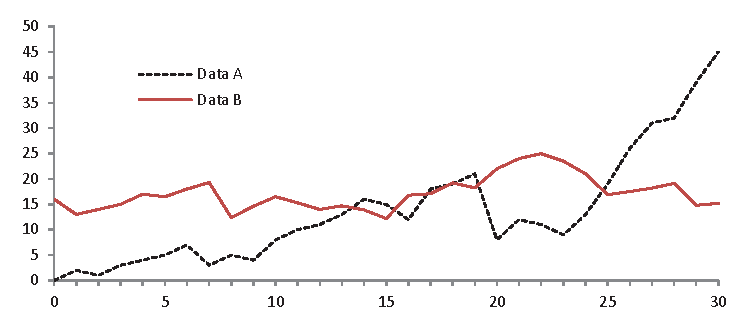
\includegraphics[width=\textwidth]{fig1.eps}
\caption{A figure caption is always placed below the illustration.
Please note that short captions are centered, while long ones are
justified by the macro package automatically.} \label{fig1}
\end{figure}

\begin{theorem}
This is a sample theorem. The run-in heading is set in bold, while
the following text appears in italics. Definitions, lemmas,
propositions, and corollaries are styled the same way.
\end{theorem}
%
% the environments 'definition', 'lemma', 'proposition', 'corollary',
% 'remark', and 'example' are defined in the LLNCS documentclass as well.
%
\begin{proof}
Proofs, examples, and remarks have the initial word in italics,
while the following text appears in normal font.
\end{proof}
For citations of references, we prefer the use of square brackets
and consecutive numbers. Citations using labels or the author/year
convention are also acceptable. The following bibliography provides
a sample reference list with entries for journal
articles~\cite{gonzalez-beltran_data_2018}, an LNCS chapter~\cite{gregory_todd_williams_sparql_2013}, a
book~\cite{ref_book1}, proceedings without editors~\cite{knublauch_shapes_2017},
and a homepage~\cite{knublauch_shapes_2017}. Multiple citations are grouped
\cite{gonzalez-beltran_data_2018,gregory_todd_williams_sparql_2013,knublauch_shapes_2017}.
%
% ---- Bibliography ----
%
% BibTeX users should specify bibliography style 'splncs04'.
% References will then be sorted and formatted in the correct style.
%
\bibliographystyle{splncs04}
\bibliography{GeoSPARQL}
%
% \begin{thebibliography}{8}
% \bibitem{ref_article1}
% Author, F.: Article title. Journal \textbf{2}(5), 99--110 (2016)

% \bibitem{ref_lncs1}
% Author, F., Author, S.: Title of a proceedings paper. In: Editor,
% F., Editor, S. (eds.) CONFERENCE 2016, LNCS, vol. 9999, pp. 1--13.
% Springer, Heidelberg (2016). \doi{10.10007/1234567890}

% \bibitem{ref_book1}
% Author, F., Author, S., Author, T.: Book title. 2nd edn. Publisher,
% Location (1999)

% \bibitem{ref_proc1}
% Author, A.-B.: Contribution title. In: 9th International Proceedings
% on Proceedings, pp. 1--2. Publisher, Location (2010)

% \bibitem{ref_url1}
% LNCS Homepage, \url{http://www.springer.com/lncs}. Last accessed 4
% Oct 2017
% \end{thebibliography}
\end{document}
